\documentclass{article}
\usepackage[utf8]{inputenc}

\title{Tesina Distributed FS (main)}
\author{alessiocorrado99 }
\date{September 2020}

\usepackage{natbib}
\usepackage[utf8]{inputenc} %input chars
\usepackage[english]{babel} %language
\usepackage[T1]{fontenc} %output chars
\usepackage{lmodern} %font
\usepackage{geometry} %page layout
\usepackage{amsfonts} %math symbols
\usepackage{amsmath} %math equations
\usepackage{amssymb} %math symbols
\usepackage{mathtools} %other math
\usepackage{paralist} %lists
\usepackage{graphicx}
\usepackage{subcaption}
\usepackage{multirow}
\usepackage{verbatim}
\usepackage{multicol}
\usepackage{pgfplots} %plots
\usepackage{listings} %listings
\usepackage[outdir=./images]{epstopdf} %eps images
\usepackage{color} %colored text
\usepackage{algorithm2e}
\usepackage{float} %images going to end of the document
\usepackage{hyperref}
\makeatletter
\newcommand{\HEADER}[1]{\ALC@it\underline{\textsc{#1}}\begin{ALC@g}}
	\newcommand{\ENDHEADER}{\end{ALC@g}}
\makeatother
\usepackage{microtype} %better type
% questo sono i default per i listings 
\lstset{
	frame=tb, % draw a frame at the top and bottom of the code block
	tabsize=4, % tab space width
	showstringspaces=false, % don't mark spaces in strings
	breaklines=true,
	numbers=left, % display line numbers on the left
	basicstyle=\footnotesize,
	commentstyle=\color{green}, % comment color
	keywordstyle=\color{blue}, % keyword color
	stringstyle=\color{red} % string color
}

\DeclareRobustCommand{\univsc}[1]{\Large\textsc{\textls[75]{#1}}}
\DeclareRobustCommand{\titlesc}[1]{\linespread{1.2}\LARGE{\textls[35]{\uppercase{#1}}\linespread{1}}}
\DeclareRobustCommand{\namesc}[1]{\large\textsc{\textls[35]{#1}}} 

\newcommand{\facciatabianca}{\newpage\shipout\null}

\allowdisplaybreaks

\begin{document}

\maketitle

\section{Introduzione}

Lo scopo del progetto è di realizzare un file system distributito. 
Le caratteristiche che deve avere sono: efficienza, accesso concorrente, replicazione dei dati (files), replicazione dei metadati (struttura del fs).

Il numero di repliche di un file è proporzionale all'importanza di esso: file con dati critici hanno numero di copie maggiore, per garantire maggiore tolleranza ai guasti e tempo di accesso minore.

Viene effettuato anche un bilanciamento del carico: i file vengono copiati o spostati in modo da non sovraccaricare un singolo server. 



\section{Architettura del sistema}

Verranno analizzate diverse possibili architetture del sistema.

\subsection{Single-server}

La prima idea è quella di avere un singolo server, il quale memorizza sia il fs che i dati. Il client interagisce direttamente con esso sia per l'esecuzione di comandi sul fs che per la memorizzazione dei dati.

Il fs viene memorizzato direttamente a partire da una directory del server, oppure in una partizione separata. In questo modo il sistema operativo si occupa direttamente della sua gestione.

La replicazione dei dati avviene mediante il salvataggio in diversi dispositivi di memorizzazione (es HDD). Per far ciò la scelta più consona è di utilizzare un sistema RAID 10: i dati vengono salvati in copia (RAID 1) per avere tolleranza ai guasti e in striping (RAID 0) per aumentare la velocità di lettura. 

Con schede di rete (e connessioni) multiple è possibile aumentare la tolleranza sia ai guasti che alle congestioni di rete. 

Vantaggi: semplice da implementare. economico. il fs è gestito direttamente dal sistema operativo. buona sicurezza contro attacchi hacker. con gli accorgimenti sopra descritti si ha già una buona robustezza.  

Svantaggi: single point of failure per quanto riguarda il server (i dati sono parzialmente protetti dal meccanismo RAID). nessuna protezione per eventi eccezionali (eg. catastrofe naturale, incendio nell'edificio, blocco della rete\dots). 

\begin{figure}[H]
	\centering
	\begin{subfigure}{0.80\linewidth}
		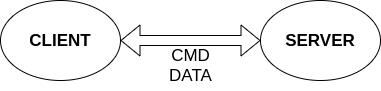
\includegraphics[width=\linewidth]{../diagrams/architettura/1.png}
	\end{subfigure}
\end{figure}



\subsection{Virtual server}

La soluzione single-server può essere migliorata aggiungendo un livello di virtualizzazione. 
Il sistema operativo non viene quindi eseguito direttamente sull'hardware ma all'interno di un container/VM. 

La macchina virtuale viene periodicamente copiata (interamente o in modo incrementale) e salvata in un dispositivo di memorizzazione dedicato. 

Nel caso ci fosse un crash o errore critico del sistema operativo, basta ricaricare la macchina virtuale più recente. La perdita di dati è limitata all'età dell'ultimo backup. 


Vantaggi: recovery buona e in tempi brevi in caso di crash. 

Svantaggi: durante il periodo di transizione il sistema non risponde. prestazioni leggermente ridotte a causa della virtualizzazione.

\begin{figure}[H]
	\centering
	\begin{subfigure}{0.80\linewidth}
		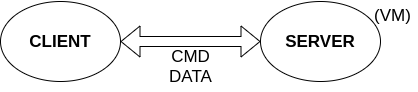
\includegraphics[width=\linewidth]{../diagrams/architettura/2.png}
	\end{subfigure}
\end{figure}



\subsection{Cloud backup}

Il backup può essere effettuato nel cloud, al posto che in un dispositivo dedicato all'interno del datacenter. Inoltre il backup può essere esteso anche ai dati, oltre che al fs. 


Vantaggi: protezione in caso di eventi eccezionali. 

Svantaggi: in generale effettuare un backup nel cloud, anche se solo incrementale, richiede un elevato utilizzo di banda e tempi maggiori. costi maggiori. 

\begin{figure}[H]
	\centering
	\begin{subfigure}{0.80\linewidth}
		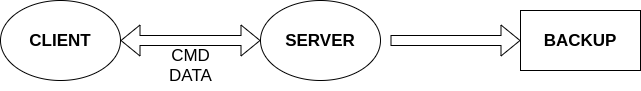
\includegraphics[width=\linewidth]{../diagrams/architettura/3.png}
	\end{subfigure}
\end{figure}



\subsection{Server as distributed database}

Al posto di utilizzare il file system del sistema operativo, è possibile utilizzare un database distribuito. Sia metadati che dati vengono salvati automaticamente nei nodi, garantendo consistenza e fault tolerance. 

Vantaggi: è possibile utilizzare un dbms in commercio, beneficiando dall'avere tutto già pronto e costantemente aggiornato.

Svantaggi: la connessione avviene tra il client ed un nodo, il quale poi distribuisce i dati agli altri nodi. se questo nodo dispone di una banda limitata, ciò può rappresentare un bottleneck dal punto di vista delle prestazioni. 

\begin{figure}[H]
	\centering
	\begin{subfigure}{0.80\linewidth}
		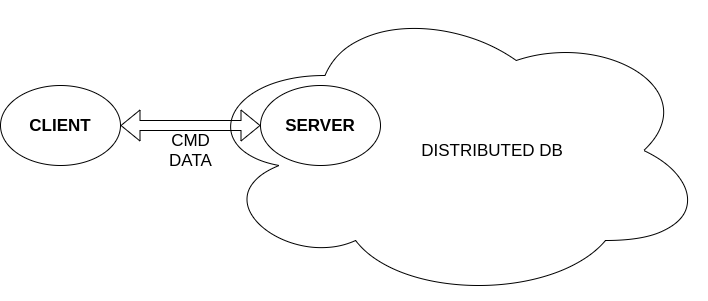
\includegraphics[width=\linewidth]{../diagrams/architettura/4.png}
	\end{subfigure}
\end{figure}



\subsection{Meta+Data server}

L'idea è di far comunicare direttamente il client con i server in cui verranno memorizzati i dati. 

Un primo sviluppo è quello di separare i compiti: si hanno quindi un "meta server" e uno o più "data server". 

Il meta server si occupa di memorizzare e gestire il file system (metadati), mentre i data server memorizzano soltanto i dati conenuti nei file. 

Per effettuare una qualsiasi operazione su un file il client si rivolge inizialmente al meta server, dal quale ottiene la configurazione per contattare il giusto data server e trasferire i dati. 

In questo modo ci sono due comunicazioni bidirezionali: client-meta, per la gestione del fs; client-data, per il trasferimento dei dati.

Per migliorare le prestazioni, soprattutto nel caso in cui il client abbia una banda più ampia rispetto ai data server, i file di grandi dimensioni vengono spezzati in chunks e distribuiti. 

Come prima il meta server è unico, virtualizzato e sottoposto a backup periodico. 

Vantaggi: connessioni a data server multipli permettono di migliorare le prestazioni nel caso in cui il client abbia una banda elevata. un unico meta server permette di mantenere in modo semplice la consistenza del file system. 

Svantaggi: la frequenza dei backup del meta server è fondamentale per minimizzare la perdita di dati in caso di fault. tutti i data server devono essere raggiungibili dal client (maggiore attenzione alla sicurezza e struttura della rete). 

\begin{figure}[H]
	\centering
	\begin{subfigure}{0.80\linewidth}
		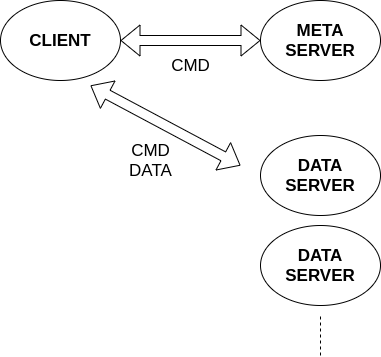
\includegraphics[width=\linewidth]{../diagrams/architettura/5.png}
	\end{subfigure}
\end{figure}



\subsection{Meta+Data server, direct config}

Facendo dialogare meta e data server, è possibile:
spostare l'onere di configurazione dei data server da client a meta server;
gestire in qualsiasi momento la replicazione dei dati, per bilanciare il carico o far fronte alla perdita di un nodo;

Il client quindi si limita a trasferire i dati da/verso data server utilizzando token forniti dal meta server. 

Vantaggi: il sistema può riconfigurarsi in ogni momento per far fronte a qualsiasi evenienza. ruolo del client semplificato. maggiore sicurezza perchè il client non può inviare comandi ai data server.

Svantaggi: maggiore complessità nel gestire operazioni concorrenti e asincrone. 

\begin{figure}[H]
	\centering
	\begin{subfigure}{0.80\linewidth}
		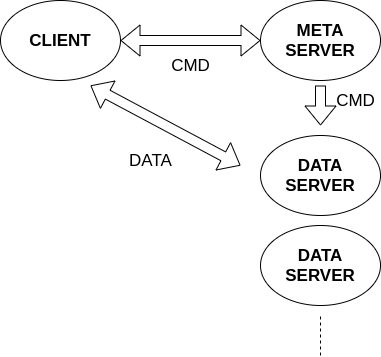
\includegraphics[width=\linewidth]{../diagrams/architettura/6.png}
	\end{subfigure}
\end{figure}



\subsection{Meta server as distributed system}

In questa soluzione non è presente un unico meta server, ma viene utilizzato un sistema distribuito. 
Approcci possibili sono utilizzare database distribuiti, blockchain o implementare a basso livello meccanismi di elezione e mantenimento della consistenza. 

Come dimostrato dal teorema CAP bisogna rinunciare alla disponibilità per garantire la coerenza del fs. 

Vantaggi: possibilità di utilizzo di software in commercio. maggiore consistenza e fault tolerance dei metadati. 

Svantaggi: maggiore difficoltà nell'implementazione dei meta server e dei protocolli di comunicazione tra i vari componenti. 

\begin{figure}[H]
	\centering
	\begin{subfigure}{0.80\linewidth}
		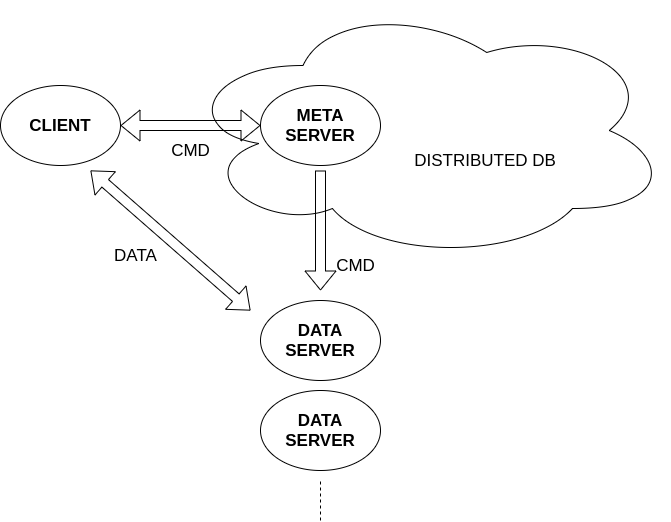
\includegraphics[width=\linewidth]{../diagrams/architettura/7.png}
	\end{subfigure}
\end{figure}


\section{Comandi}


\subsection{Comandi del client}

list <path?> <-r> <-meta> <-format={json, csv, default}>:
lista il contenuto di una cartella. output per linea
dir=path assoluto. se assente root.
-r=ricorsivo
-meta=includi metadati
-format=formato output

mkdir <path>
crea una cartella

meta <path>
metadati di un path

get <path>
download di un file

push <path> 
upload di un file

rem <path>
delete di un path

link <file path> <link path> 
crea link 


\subsection{Metadati dei path}

I metadati associati ad un path sono: 

uid = usato come identifcatore univoco anche per versioni dello stesso path

name

creation date

size

owner = chi l'ha creato è owner

visible = visibile solo da owner o pubblico

ncopies = numero copie minimo desiderato


\section{Protocollo comunicazione}

Di seguito i flussi di dati coinvolti nelle diverse tipologie di richieste.

\subsection{get}

La richiesta di tipo \textit{get(path)} richiede il trasferimento in entrata di un file. 

Inizialmente il \textit{client} contatta il \textit{meta server}, richiedendo un particolare \textit{path}. Il \textit{meta server} seleziona il \textit{data server} ottimale per gestire la richiesta (deve contenere la risorsa e non essere sovraccarico). Il \textit{meta server} risponde quindi al client specificando l'uid della risorsa (richiesto per identificarla) e l'indirizzo del \textit{data server} a cui collegarsi. Il \textit{client} si disconnette dal \textit{meta server}.

Il \textit{client} si connette al \textit{data server} inviando una richiesta \textit{get(uid)}. Se la risorsa è disponibile (come dovrebbe essere) il \textit{data server} invia un \textit{ack} seguito dal flusso di dati del file. (TODO implementare lastpos) Altrimenti risponde con \textit{err} seguito dai dettagli. 

\begin{figure}[H]
	\centering
	\begin{subfigure}{0.80\linewidth}
		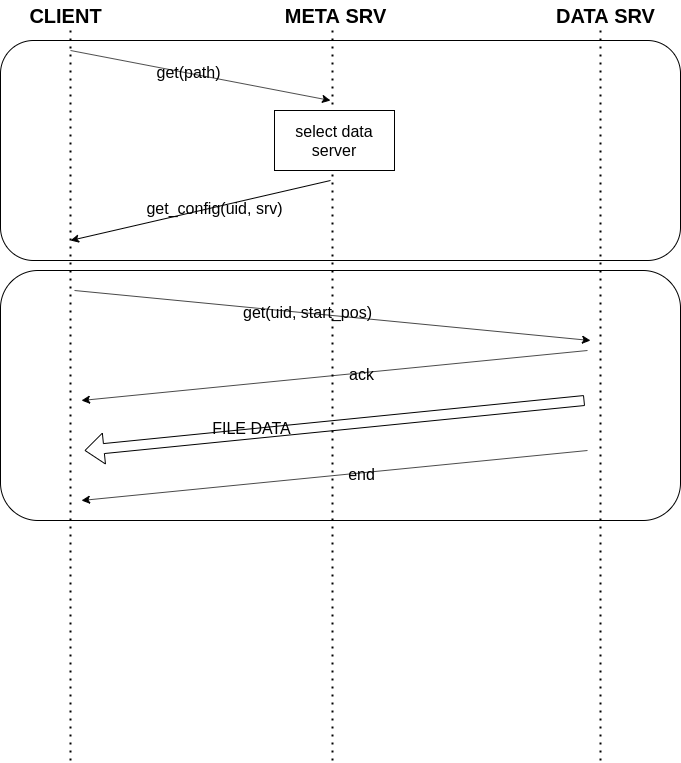
\includegraphics[width=\linewidth]{../diagrams/requests/get_request.png}
	\end{subfigure}
\end{figure}


\subsection{push}

La richiesta di tipo \textit{push(path, data)} richiede il trasferimento in uscita di un file da parte del client. 

Inizialmente il \textit{client} contatta il \textit{meta server}, inviando \textit{path} e \textit{size}. Il \textit{meta server} seleziona il \textit{data server} ottimale per gestire la richiesta (deve poter contenere la risorsa e non essere sovraccarico). Il \textit{meta server} si occupa anche di generare un nuovo \textit{uid} da assegnare alla risorsa. 

Il \textit{meta server} si collega al \textit{data server} dove verrà inizialmente salvata la risorsa, inviando un comando \textit{create(uid, size)}. Questo comando predispone il \textit{data server} per ospitare un nuovo documento con tale uid. Se non ci sono errori, il \textit{data server} risponde al \textit{meta server} con \textit{ack}. Altrimenti con \textit{err} seguito dai dettagli.

(TODO aggiungi size a create)
(TODO aggiungi richieste eliminazione)

Il \textit{meta server} risponde quindi al client specificando l'uid della risorsa (richiesto per identificarla) e l'indirizzo del \textit{data server} a cui collegarsi. Il \textit{client} si disconnette dal \textit{meta server}.

Inizia quindi il caricamento del documento. Il \textit{client} si collega al \textit{data server} e invia una \textit{push(uid)}. Se non ci sono errori, il \textit{data server} risponde con \textit{ack} e invia la posizione (indice 0-based) \textit{last\_pos} del primo byte non trasferito (equivalente al numero di byte già trasferiti). A quel punto il \textit{client} trasferisce la porzione rimanente di documento. Al termine del trasferimento, se non ci sono errori, il \textit{data server} risponde con \textit{ack}. La connessione viene chiusa.

Quando il trasferimento è completato con successo, inizia la terza fase. Il \textit{data server} invia un messaggio del tipo \textit{push\_complete(uid)} al \textit{meta server}. Il meta server inizia quindi ad inviare ai \textit{data server} interessati le richieste di trasferimento, per raggiungere il grado di replicazione voluto.

(TODO aggiungi richieste trasferimento)

\begin{figure}[H]
	\centering
	\begin{subfigure}{0.80\linewidth}
		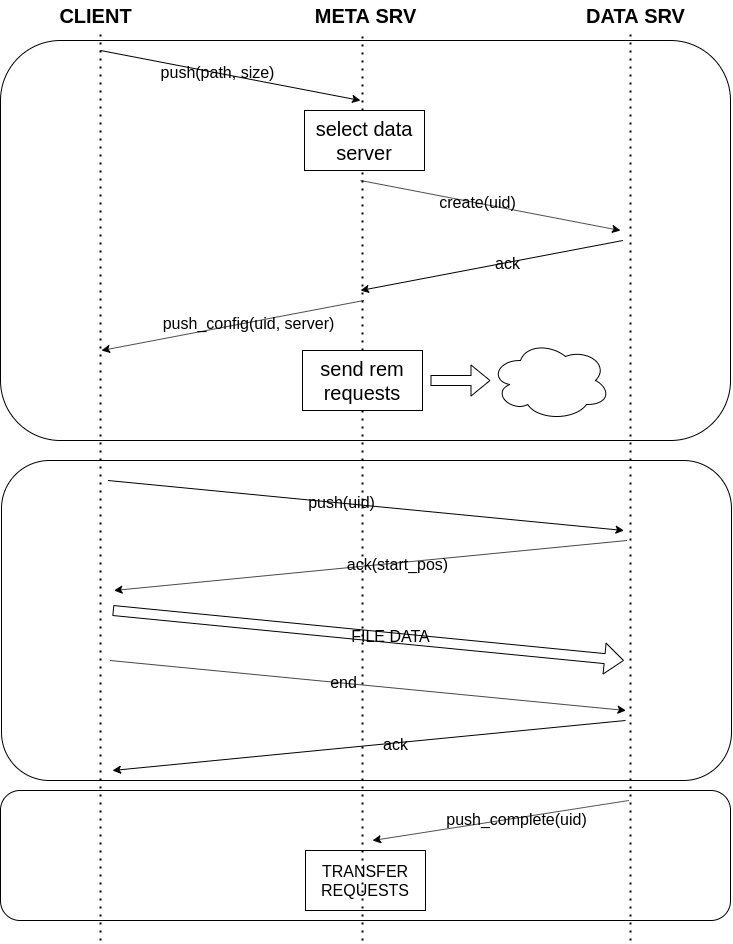
\includegraphics[width=\linewidth]{../diagrams/requests/push_request.png}
	\end{subfigure}
\end{figure}


\subsection{rem}

La richiesta di tipo \textit{rem(path)} richiede l'eliminazione di un file/directory dallo storage.

Il \textit{client} invia al \textit{meta server} una richiesta \textit{rem(path)}. Se non ci sono errori, il \textit{meta server} risponde con \textit{ack} e chiude la connessione.

Il \textit{meta server} contatta separatamente tutti i \textit{data server} contenenti dati relativi a quel particolare \textit{uid} e invia una richiesta \textit{rem(uid)}.  

\begin{figure}[H]
	\centering
	\begin{subfigure}{0.80\linewidth}
		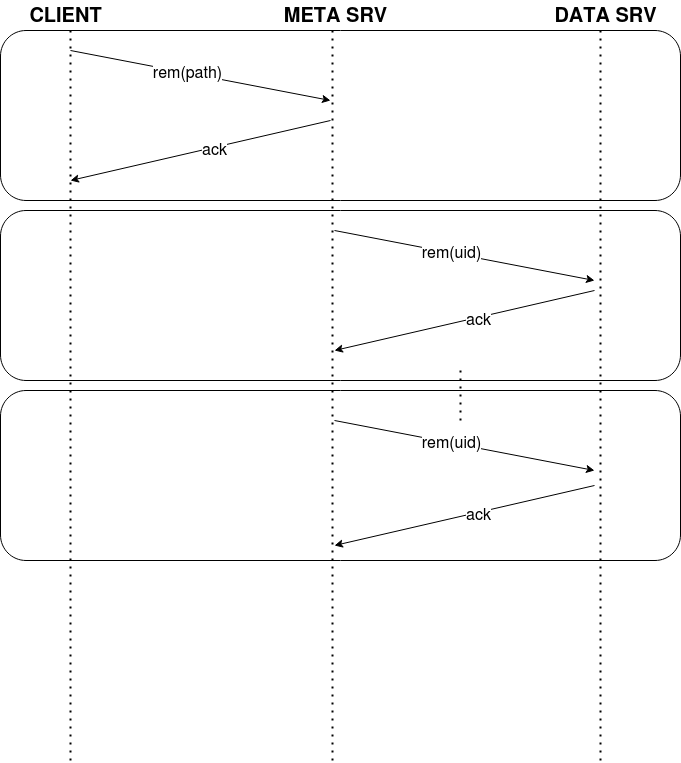
\includegraphics[width=\linewidth]{../diagrams/requests/rem_request.png}
	\end{subfigure}
\end{figure}



\subsection{transfer}

(TODO fai tutto)


\begin{figure}[H]
	\centering
	\begin{subfigure}{0.80\linewidth}
		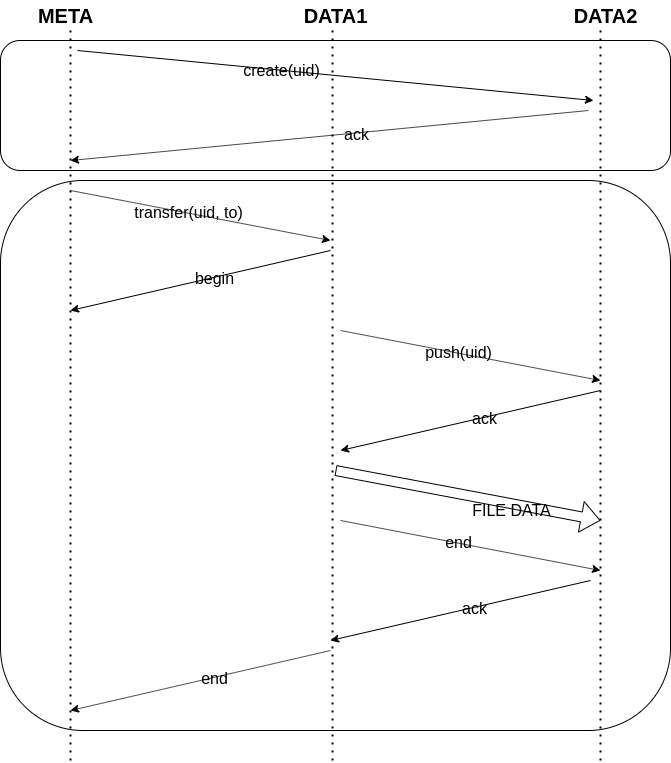
\includegraphics[width=\linewidth]{../diagrams/requests/transfer_request.png}
	\end{subfigure}
\end{figure}




\section{Logging}

Tutte le operazioni prima di essere eseguite vengono registrate in appositi database di log. In questo modo, se un'operazione viene interrotta per qualsiasi motivo, può essere analizzata e rieseguita, in modo da non lasciare spazzatura. 



\bibliographystyle{plain}
\bibliography{references}
\end{document}
